\documentclass[12pt]{article}%
\usepackage{graphics, graphicx, cite, fancybox, setspace}
\usepackage{color}
\usepackage{boxedminipage}
\usepackage{amsfonts,amssymb,amsmath}
\usepackage{url}
\usepackage{wrapfig,sectsty}
\usepackage[letterpaper, left=1in, right=1in, top=1in, bottom=1in]{geometry}
\usepackage{multirow}
\usepackage{times}
\usepackage{verbatim}
\usepackage{epsfig}
\usepackage{subcaption}

%
\usepackage{array}
\usepackage{rotating}


\usepackage{enumitem}
\usepackage{float}
\usepackage{titlesec}







%%%%%%%%%%%%%%%%%%%%%%%%%%%%%%%%%%%%%%%%%%%%%%%%%%%%%%%


\titleformat{\section}
  {\normalfont\fontsize{14}{1em}\bfseries}{\thesection}{1em}{}

%%%%%%%%%%%%%%%%%%%%%%%%%%%%%%%%%%%%%%%%%%%%%%%%%%%%%%%

\def\bi{\begin{itemize}     % Begin Itemize
\vspace{-0.5em}\setlength\itemsep{0em}}

%%%%%%%%%%%%%%%%%%%%%%%%%%%%%%%%%%%%%%%%%%%%%%%%%%%%%%%


\begin{document}

\begin{center}
{\LARGE 04/22/19 Weekly Report}\\
\vspace{0.5em}
{\Large Hunter Kippen}
\vspace{0.5em}
\end{center}


\section{What I worked on last week}
\bi
\item I attempted to optimize the SVM classifier. I first looked at the effect of selectively adding different AR models to the feature set supplied to the SVM. The ROC curves are found in Fig. ~\ref{FeatComp}
\item After this, I attempted to use the Radial Basis Function Kernel instead of a linear kernel. The rbf kernel did not work the greatest out of the box, so I followed Owen's advice and swept through different values for C and $\gamma$. Figures ~\ref{logsearch}, and ~\ref{linsearch} show the accuracy as a surface plot versus C and $\gamma$. 

An interesting thing to note is that the optimal value is when $\gamma$ is very small. I'm not sure this is what we want to use. As shown in Fig. ~\ref{rbfcomp}, a linear kernel may still be best. I believe this warrants further exploration, but I'm not necessarily sure how to go about it. 
\end{itemize}


\begin{figure}[htbp]
\centerline{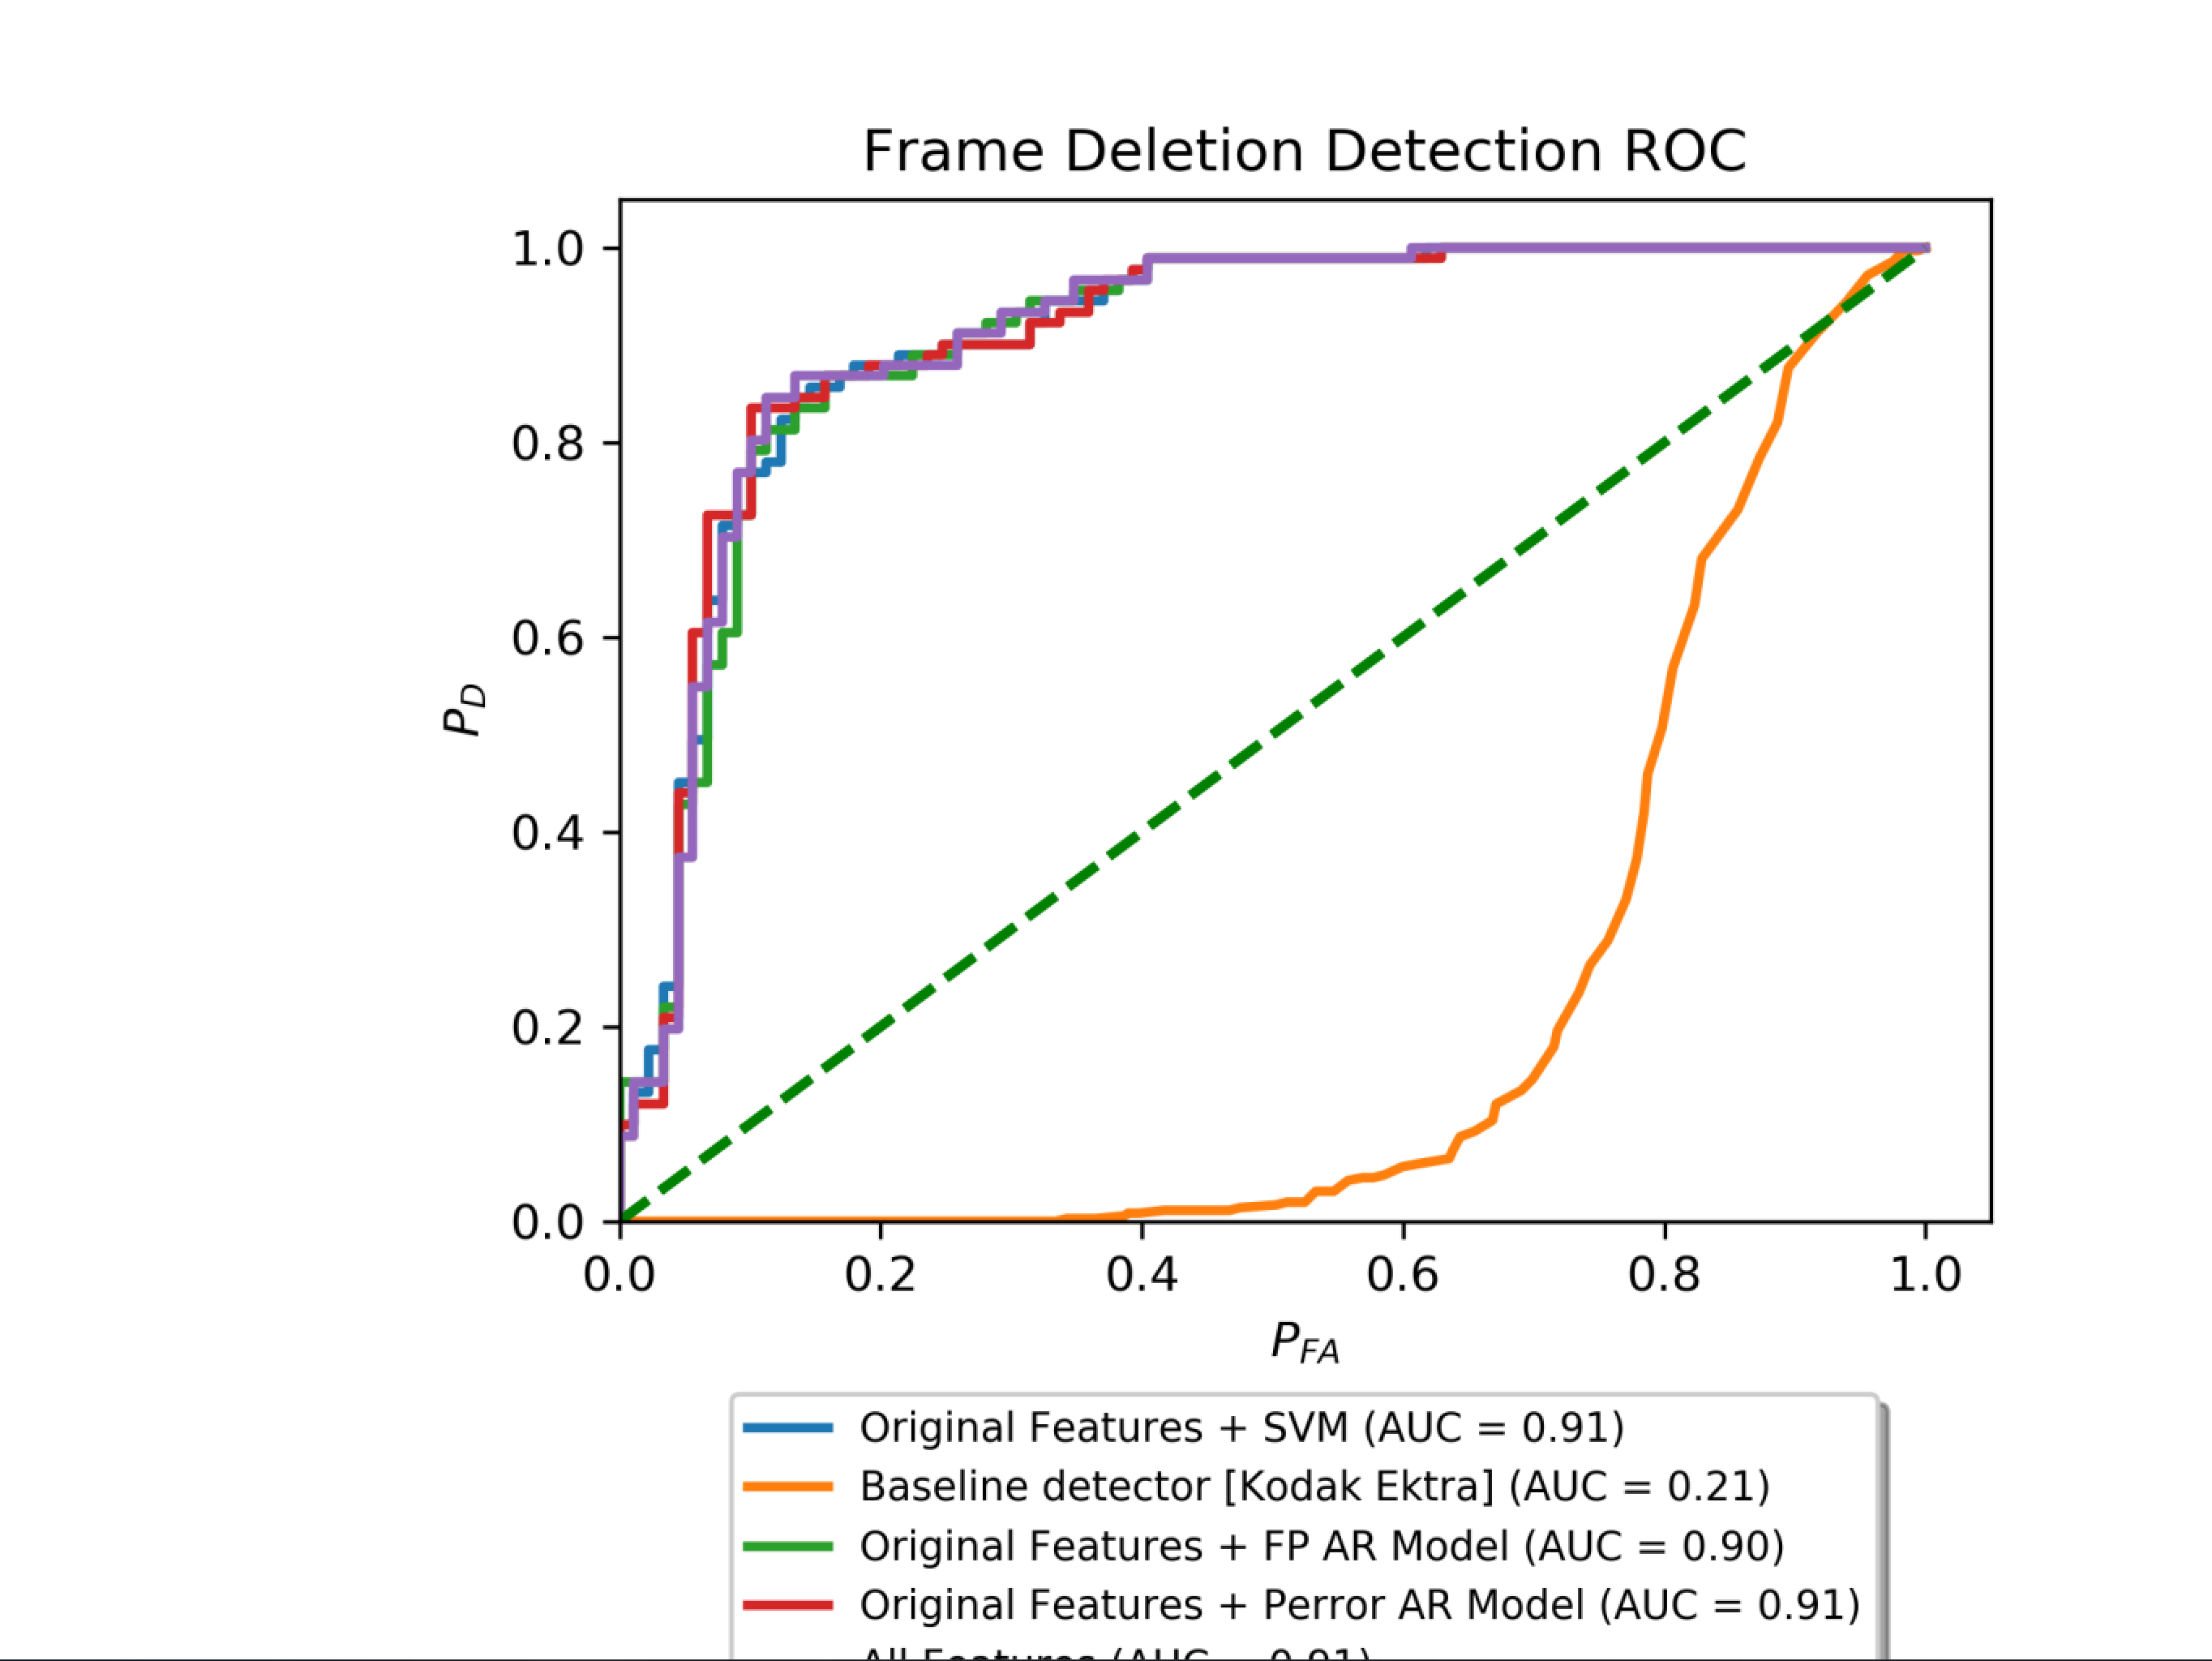
\includegraphics[width=0.9\linewidth]{../Graphs/perror_all_AR_model_comparison.png}}
\caption{Graph of SVM ROC Curves for SVMs Using Various Combinations of Features}
\label{FeatComp}
\end{figure}

\begin{figure}[htbp]
\centerline{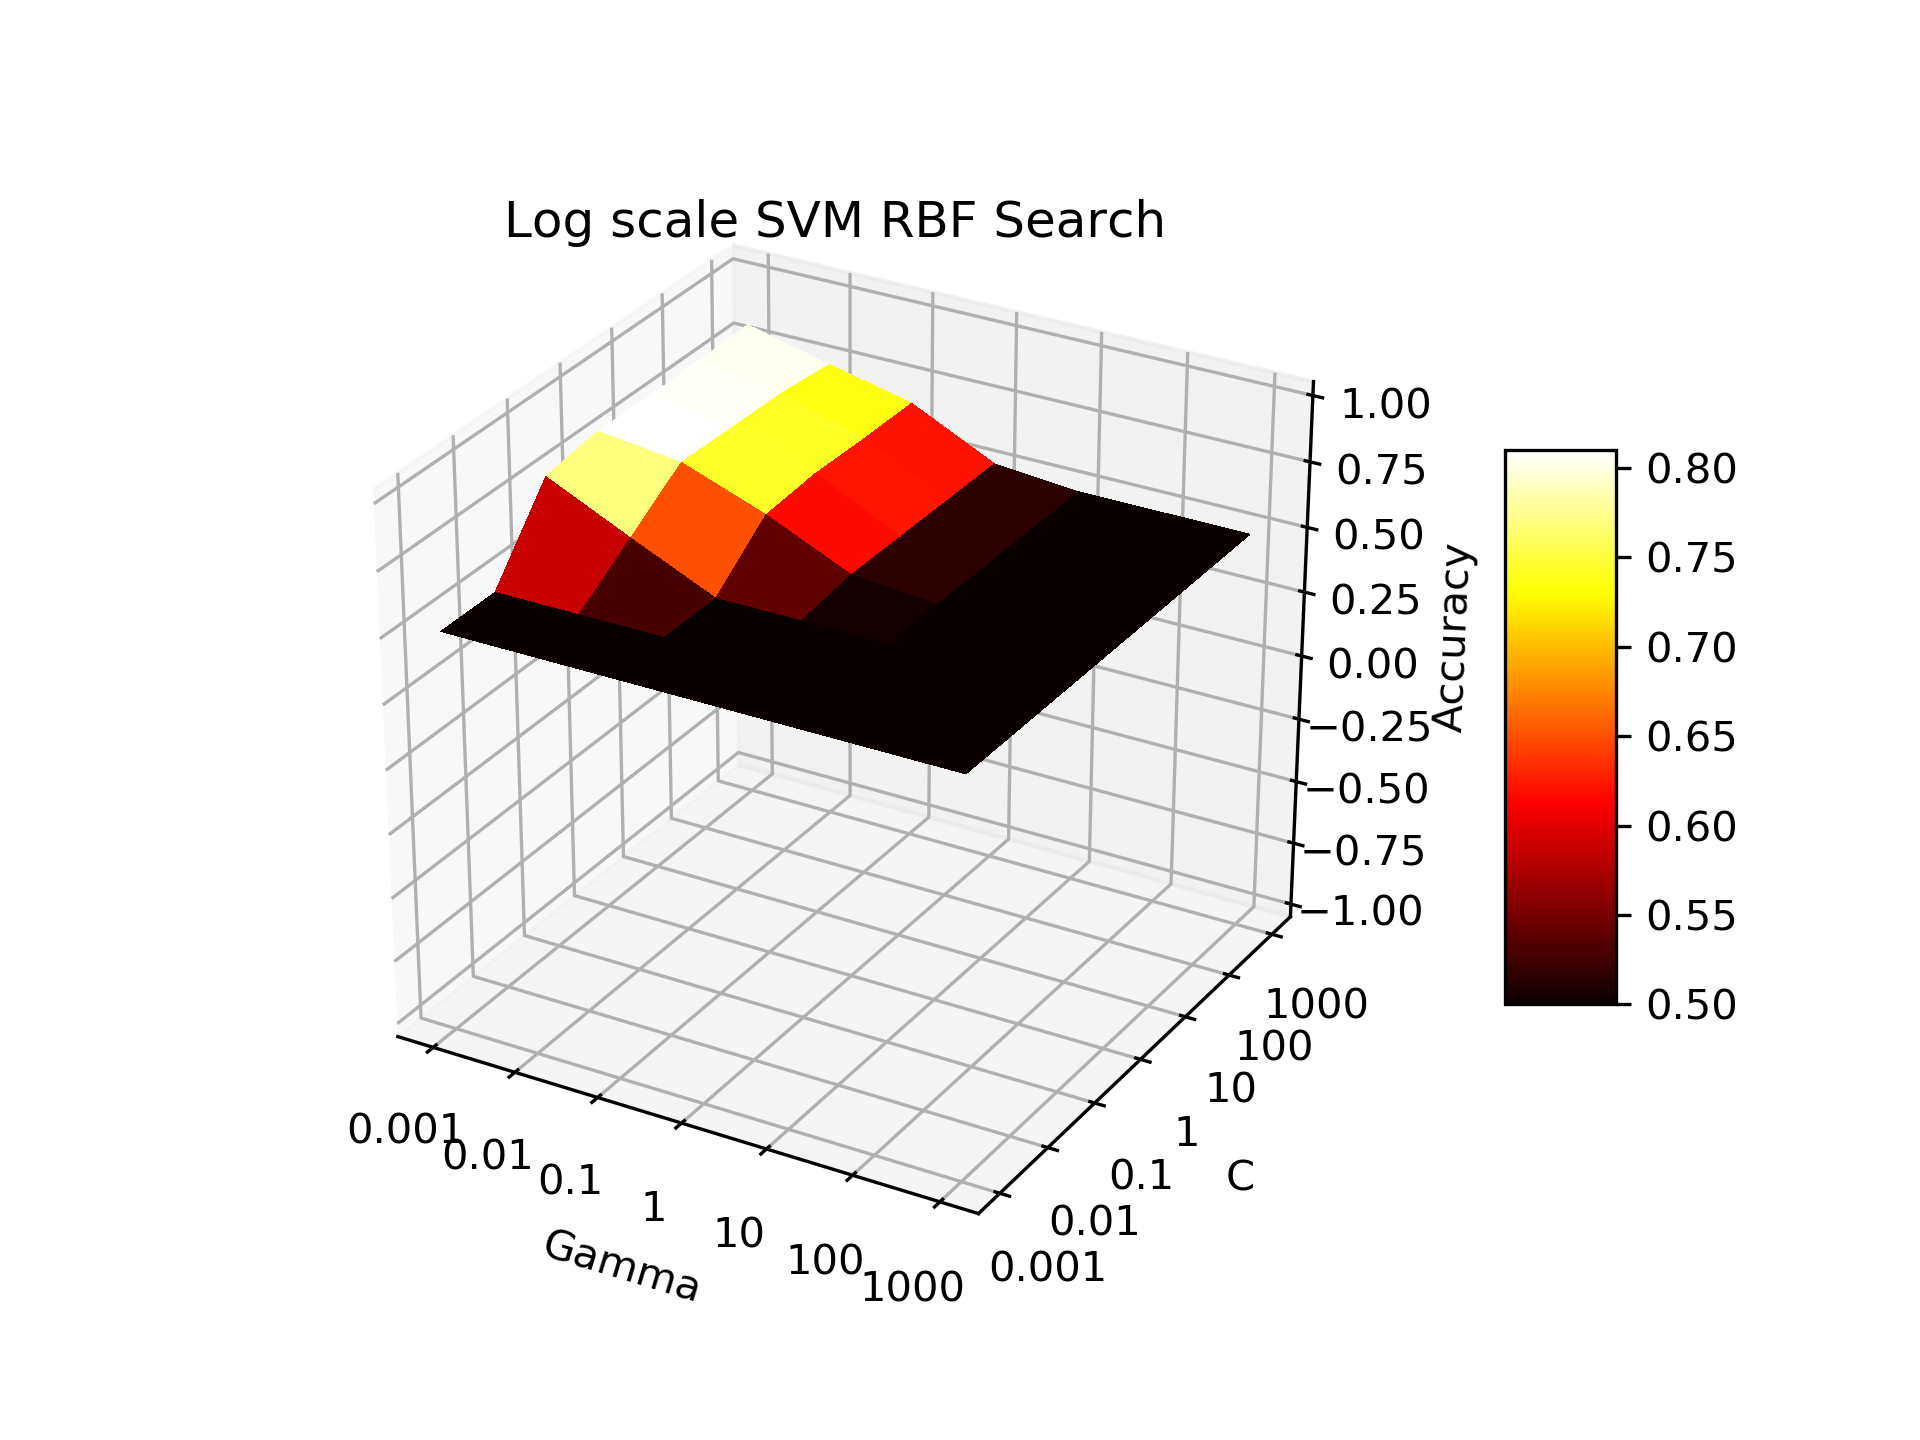
\includegraphics[width=0.9\linewidth]{../Graphs/log_scale_rbf_search.png}}
\caption{Log Scale Search for Optimal C and $\gamma$}
\label{logsearch}
\end{figure}

\begin{figure}[htbp]
\centerline{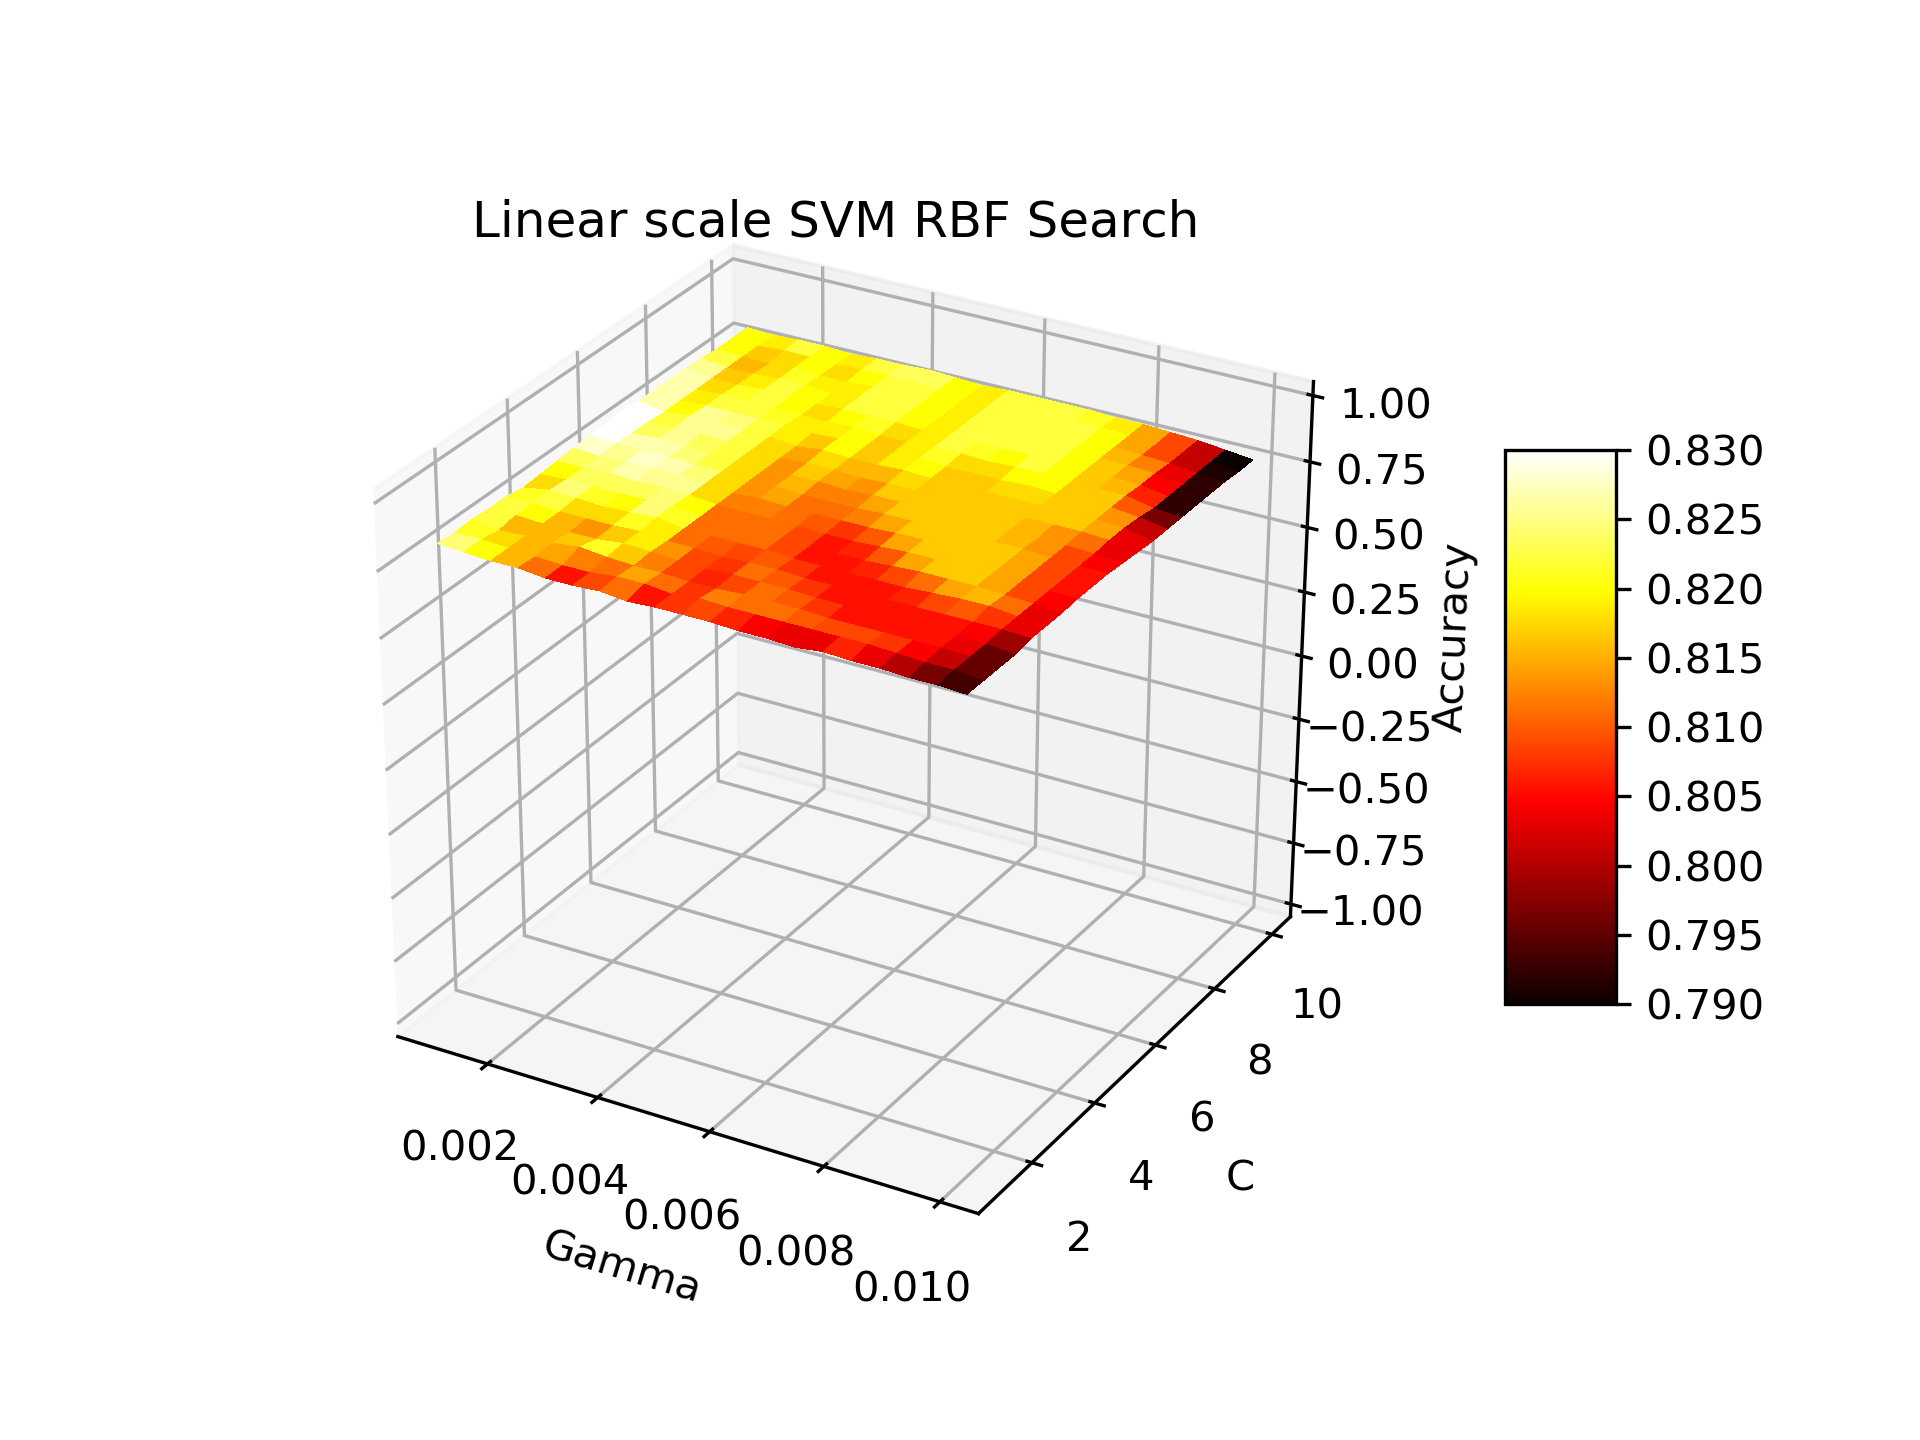
\includegraphics[width=0.9\linewidth]{../Graphs/linear_scale_rbf_search.png}}
\caption{Linear Scale Search for Optimal C and $\gamma$}
\label{linsearch}
\end{figure}

\begin{figure}[htbp]
\centerline{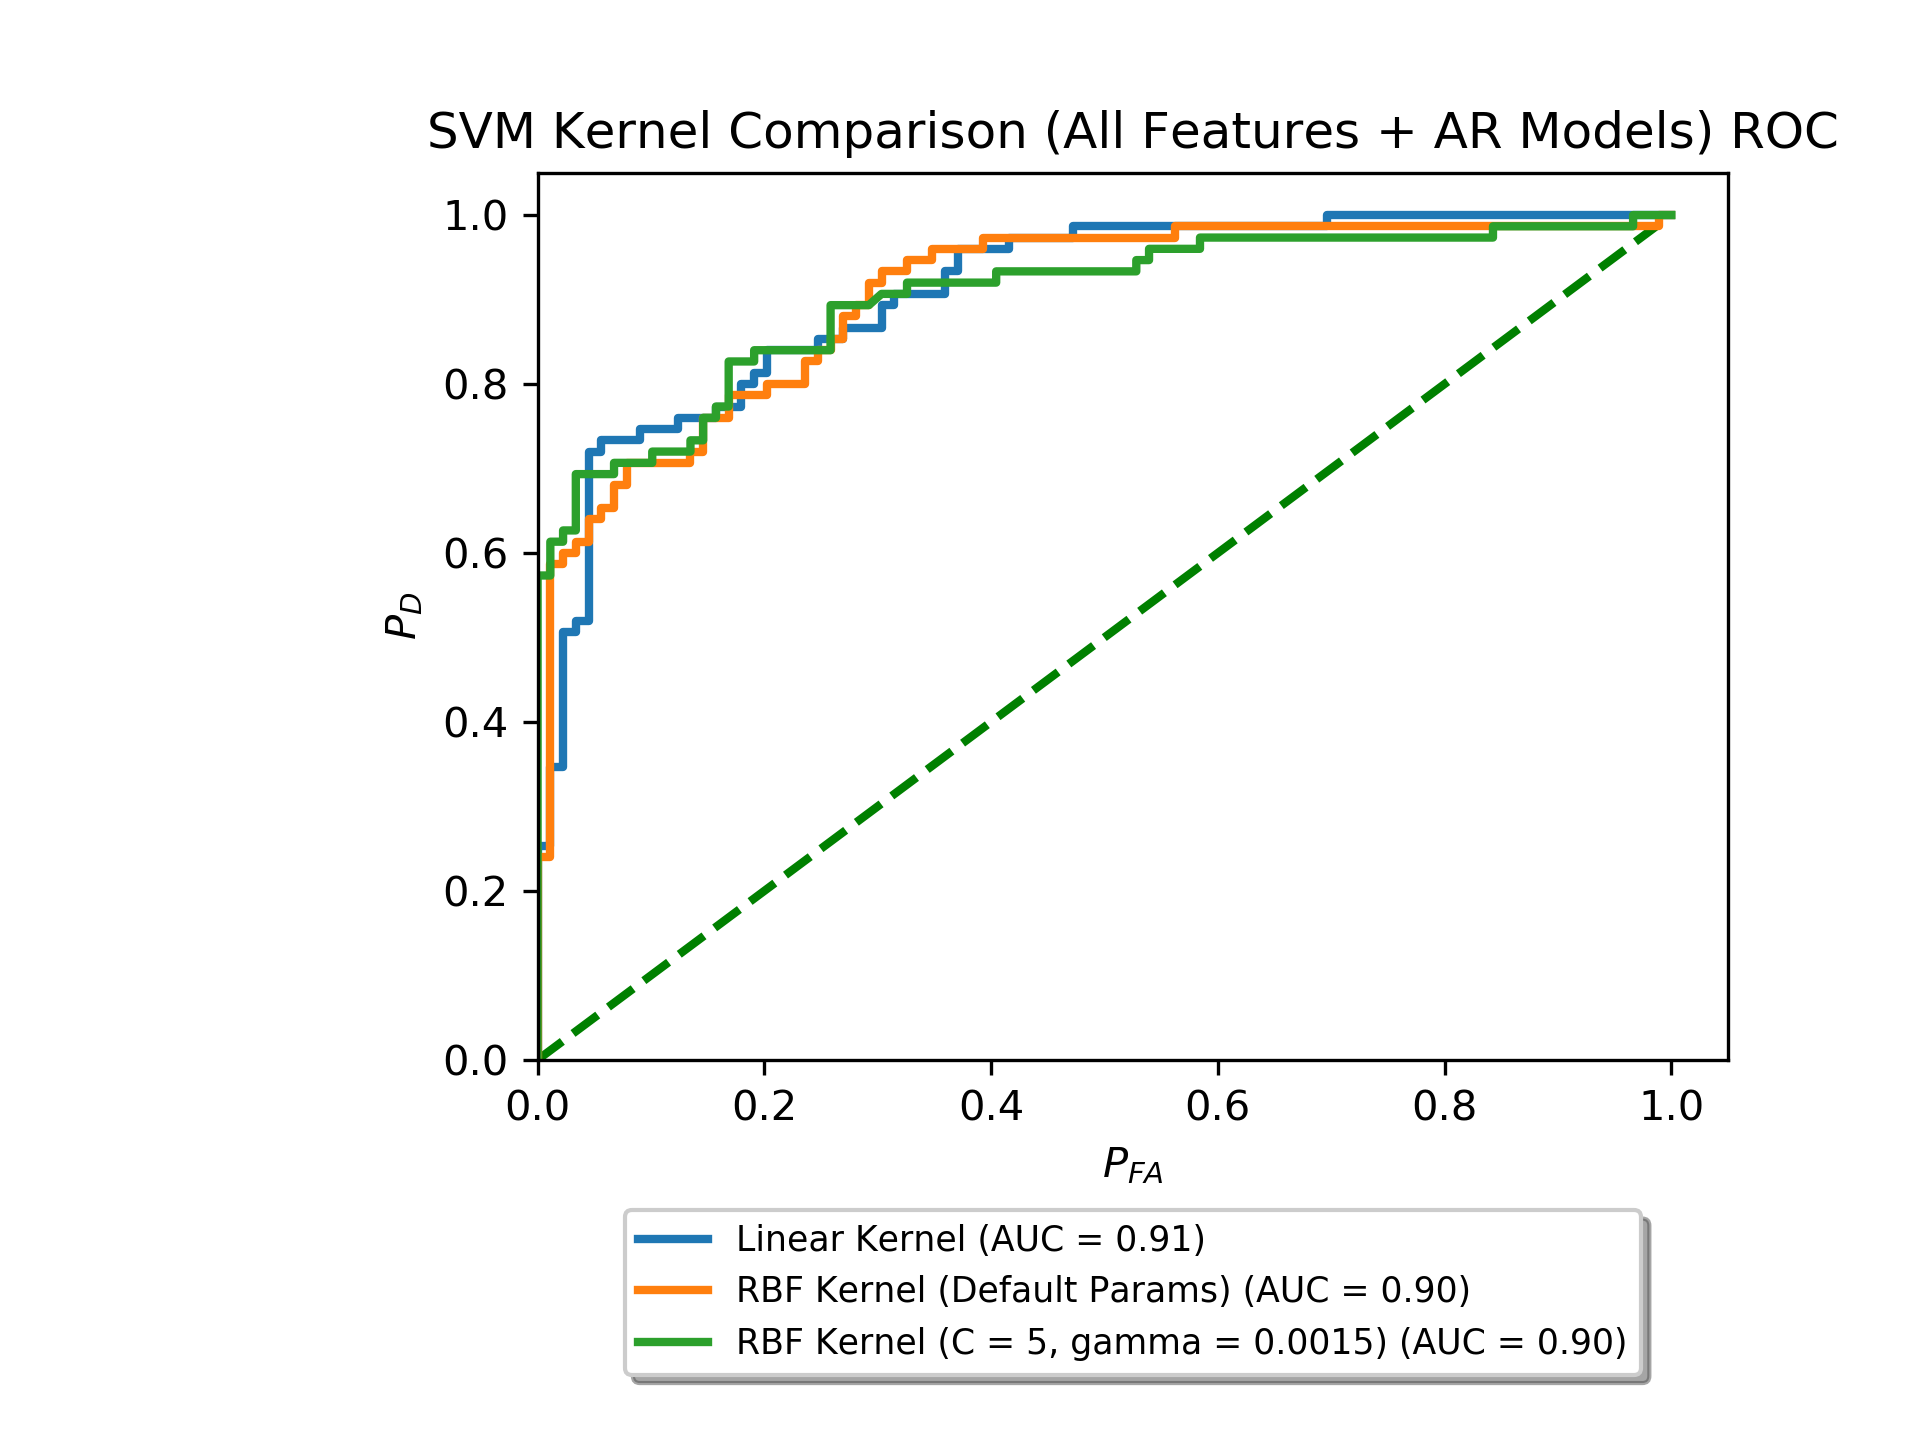
\includegraphics[width=0.9\linewidth]{../Graphs/SVM_kernel_comparison_roc.png}}
\caption{Different SVM Kernel Parameter Comparison}
\label{rbfcomp}
\end{figure}

\section{Problems I encountered}
\bi
\item Regardless of relative performance, I do not believe we are quite there on overall accuracy for the detector. The paper by Barni where they explore the inconsistencies in the number of skip blocks gets over 90\% accuracy for detecting both deletion and insertion, and it's localized!. At this point, I am not sure how we can match or exceed that.
\end{itemize}

\section{What I plan to do this week}
\bi
\item I plan to explore how the current detector fairs on a combined dataset of multiple camera models. I believe it is imperative that we nail down how different initial conditions affect the detector. If the detector can generalize for say 5 different camera models, then I believe we have good features. Otherwise, some tweaks in methodology or algorithms may be necessary.
\item Once we determine that, I am going to update my C code to account for B-frames, and perform similar experiments on datasets where the cameras have varied GOP structure.
\end{itemize}


% Bib/refs go here if used

\begin{comment}
\pagebreak
%\bibliographystyle{plain}
\bibliographystyle{myIEEE}
\bibliography{StammRefs}
%\bibliography{StammRefs,kandasamy_v2,kandasamy}
\end{comment}


\end{document} 